\documentclass[12pt, a4paper, oneside]{ctexart}
\usepackage{amsmath, amsthm, amssymb, bm, color, graphicx, geometry, hyperref, mathrsfs,extarrows, braket, booktabs, array, listings, xcolor, fontspec, appendix, numprint}
\setmonofont{Consolas}

%%%%%% 设置字号 %%%%%%
\newcommand{\chuhao}{\fontsize{42pt}{\baselineskip}\selectfont}
\newcommand{\xiaochuhao}{\fontsize{36pt}{\baselineskip}\selectfont}
\newcommand{\yihao}{\fontsize{28pt}{\baselineskip}\selectfont}
\newcommand{\erhao}{\fontsize{21pt}{\baselineskip}\selectfont}
\newcommand{\xiaoerhao}{\fontsize{18pt}{\baselineskip}\selectfont}
\newcommand{\sanhao}{\fontsize{15.75pt}{\baselineskip}\selectfont}
\newcommand{\sihao}{\fontsize{14pt}{\baselineskip}\selectfont}
\newcommand{\xiaosihao}{\fontsize{12pt}{\baselineskip}\selectfont}
\newcommand{\wuhao}{\fontsize{10.5pt}{\baselineskip}\selectfont}
\newcommand{\xiaowuhao}{\fontsize{9pt}{\baselineskip}\selectfont}
\newcommand{\liuhao}{\fontsize{7.875pt}{\baselineskip}\selectfont}
\newcommand{\qihao}{\fontsize{5.25pt}{\baselineskip}\selectfont}

%%%% 下面的命令重定义页面边距,使其符合中文刊物习惯 %%%%
\addtolength{\topmargin}{-54pt}
\setlength{\oddsidemargin}{0.63cm}  % 3.17cm - 1 inch
\setlength{\evensidemargin}{\oddsidemargin}
\setlength{\textwidth}{14.66cm}
%\setlength{\textheight}{28.00cm}    % 24.62
\setlength{\textheight}{26.00cm}    % 24.62

%%%% 下面的命令设置行间距与段落间距 %%%%
\linespread{1.4}
% \setlength{\parskip}{1ex}
\setlength{\parskip}{0.5\baselineskip}
%%%% 代码块的基本设置 %%%%
\lstset{
    language = python,
    breaklines,%自动换行
    columns=flexible,%不随便添加空格,只在已经有空格的地方添加空格,
    %如果想要添加空格使用fixed作为参数(这是默认的),如果坚决不添加空格使用fullflexible作为参数.
    numbers=left, 
    numberstyle=\footnotesize\color{darkgray},
    %numberstyle=\tiny,
    keywordstyle=\color{blue!70},
    commentstyle=\color{red!50!green!50!blue!50},
    frame=shadowbox,
    rulesepcolor=\color{red!20!green!20!blue!20},
    basicstyle=\ttfamily
}

%%%% 正文开始 %%%%
\begin{document}

%%%% 定理类环境的定义 %%%%
\newtheorem{example}{例}             % 整体编号
\newtheorem{algorithm}{算法}
\newtheorem{theorem}{定理}[section]  % 按 section 编号
\newtheorem{definition}{定义}
\newtheorem{axiom}{公理}
\newtheorem{property}{性质}
\newtheorem{proposition}{命题}
\newtheorem{lemma}{引理}
\newtheorem{corollary}{推论}
\newtheorem{remark}{注解}
\newtheorem{condition}{条件}
\newtheorem{conclusion}{结论}
\newtheorem{assumption}{假设}

%%%% 重定义 %%%%
\renewcommand{\contentsname}{目录}  % 将Contents改为目录
\renewcommand{\abstractname}{摘要}  % 将Abstract改为摘要
\renewcommand{\refname}{参考文献}   % 将References改为参考文献
\renewcommand{\indexname}{索引}
\renewcommand{\figurename}{图}
\renewcommand{\tablename}{表}
\renewcommand{\appendixname}{附录}
\renewcommand{\algorithm}{算法}


%%%% 定义标题格式,包括title,author,affiliation,email等 %%%%
\title{数值分析第二次上机试验报告\\龙贝格积分法}
\author{吴天阳\\2204210460\\59\\[2ex]
\xiaosihao 西安交通大学\\[2ex]
}
\date{2022年4月17日}

\maketitle % 设置上面是标题
\newpage
\tableofcontents % 创建目录,使用目录需要编译两次,并且不能删去编译产生的临时文件!!!

%%%% 以下部分是正文 %%%%  
\newpage
\section{问题描述}
使用龙贝格积分法计算如下四个积分,使计算结果尽可能准确。
\begin{equation*}
    \begin{aligned}
        \int_0^1\frac{1}{1+x}\,dx;\quad(2)\int_0^1\frac{\ln(1+x)}{1+x^2}\,dx;\quad(3)\int_0^1\frac{\ln(1+x)}{x}\,dx;\quad(4)\int_0^{\pi/2}\frac{\sin x}{x}\,dx.
    \end{aligned}
\end{equation*}
\section{算法实现}
直接利用Romberg积分公式,有如下递推式\begin{equation*}
    \begin{aligned}
        T_1 =&\ \frac{b-a}{2}[f(a)+f(b)],\\
        T_{2^{i}} =&\ \frac{1}{2}T_{2^{i-1}}+\frac{b-a}{2^i}\sum_{k=0}^{2^i-1}f(a+(2k+1)\frac{b-1}{2^i})&(i=1,2,\cdots)\\
        S_{2^{i}} =&\ T_{2^{i+1}}+\frac{1}{4-1}(T_{2^{i+1}}-T_{2^k})\\
        C_{2^{i}} =&\ S_{2^{i+1}}+\frac{1}{4^2-1}(S_{2^{i+1}}-S_{2^k})&(i=0,1,2,\cdots)\\
        R_{2^{i}} =&\ C_{2^{i+1}}+\frac{1}{4^3-1}(C_{2^{i+1}}-C_{2^k})\\
    \end{aligned}
\end{equation*}
使用Python的列表实现上述递推过程,构造如下列表:
\renewcommand\arraystretch{0.8} % 设置表格高度为原来的0.8倍
\begin{table}[!htbp] % table标准
    \centering % 表格居中
    \begin{tabular}{p{3cm}<{\centering}p{3cm}<{\centering}p{3cm}<{\centering}p{3cm}<{\centering}} % 设置表格宽度
    %\begin{tabular}{cccc}
        \toprule
        $T_{2^k}$ & $S_{2^k}$ & $C_{2^k}$ & $R_{2^k}$\\
        \midrule
        $T_1$ &  &                  &                          \\
        $T_2$ & $S_1$ &         &                          \\
        $T_{2^2}$ & $S_2$ & $C_1$ & \\
        $T_{2^3}$ & $S_{2^2}$ & $C_2$ & $R_1$\\
        $T_{2^4}$ & $S_{2^3}$ & $C_{2^2}$ & $R_2$\\
        $\vdots$ & $\vdots$ & $\vdots$ & $\vdots$\\
        \bottomrule
    \end{tabular}
\end{table}
\newpage
主要算法部分代码:
\begin{lstlisting}
    upper = 20  # 计算次数的上界
    table = [[(b-a)/2 * (fun(a) + fun(b))]]  # T1初始化
    for i in range(1, upper):
        tmp = 0
        for k in range(np.power(2, i-1)):
            tmp += fun(a + (2*k+1) * (b-a) / np.power(2, i))
        tmp *= (b - a) / np.power(2, i)
        table.append([1/2 * table[i-1][0] + tmp])  # 计算T_2^i
        for j in range(1, min(i, 3) + 1):  # 递归求值
            table[i].append(table[i][j-1] + (table[i][j-1]-table[i-1][j-1]) / (np.power(4, j)-1))
        if i >= 4 and np.abs(table[i][3] - table[i - 1][3]) <= eps:  # 达到精度要求
            break
    return table[i][3]
\end{lstlisting}
\section{试验结果}
\def\disp{\displaystyle}
由于Python的浮点型最多只有16位有效数字,所以计算结果误差最小只能达到$10^{-15}$。

\subsection{积分一}
截断误差为$10^{-15}$,$\disp\int_0^1\frac{1}{1+x}\,dx\approx 0.\numprint{6931471805599452}$,下表列出了前$7$次的计算结果:

\renewcommand\arraystretch{0.8} % 设置表格高度为原来的0.8倍
\begin{table}[!htbp] % table标准
\centering % 表格居中
\begin{tabular}{cccc}
\toprule
$T_{2^k}(k = 0,1,\cdots, 6)$ & $S_{2^k}$ & $C_{2^k}$ & $R_{2^k}$ \\
\midrule
 0.\numprint{750000000000} &                &                &                \\
 0.\numprint{708333333333} & 0.\numprint{694444444444} &                &                \\
 0.\numprint{697023809524} & 0.\numprint{693253968254} & 0.\numprint{693174603175} &                \\
 0.\numprint{694121850372} & 0.\numprint{693154530655} & 0.\numprint{693147901481} & 0.\numprint{693147477645} \\
 0.\numprint{693391202208} & 0.\numprint{693147652819} & 0.\numprint{693147194297} & 0.\numprint{693147183072} \\
 0.\numprint{693208208269} & 0.\numprint{693147210290} & 0.\numprint{693147180788} & 0.\numprint{693147180573} \\
 0.\numprint{693162438883} & 0.\numprint{693147182421} & 0.\numprint{693147180564} & 0.\numprint{693147180560} \\
\bottomrule
\end{tabular}
\end{table}

\subsection{积分二}
截断误差为$10^{-15}$,$\disp\int_0^1\frac{\ln(1+x)}{1+x^2}\,dx\approx 0.\numprint{27219826128795027}$,下表列出了前$7$次的计算结果:

\renewcommand\arraystretch{0.8} % 设置表格高度为原来的0.8倍
\begin{table}[!htbp] % table标准
\centering % 表格居中
\begin{tabular}{cccc}
\toprule
$T_{2^k}(k = 0,1,\cdots, 6)$ & $S_{2^k}$ & $C_{2^k}$ & $R_{2^k}$ \\
\midrule
 0.\numprint{173286795140} &                &                &                \\
 0.\numprint{248829440813} & 0.\numprint{274010322704} &                &                \\
 0.\numprint{266457611491} & 0.\numprint{272333668384} & 0.\numprint{272221891429} &                \\
 0.\numprint{270768638296} & 0.\numprint{272205647230} & 0.\numprint{272197112487} & 0.\numprint{272196719170} \\
 0.\numprint{271841192282} & 0.\numprint{272198710278} & 0.\numprint{272198247814} & 0.\numprint{272198265835} \\
 0.\numprint{272109014944} & 0.\numprint{272198289164} & 0.\numprint{272198261090} & 0.\numprint{272198261301} \\
 0.\numprint{272175951006} & 0.\numprint{272198263027} & 0.\numprint{272198261285} & 0.\numprint{272198261288} \\
\bottomrule
\end{tabular}
\end{table}

\subsection{积分三}
由于收敛速度较慢,截断误差只能为$10^{-6}$,$\disp\int_0^1\frac{\ln(1+x)}{x}\,dx\approx 0.\numprint{822466}$,下表列出了前$20$次的计算结果:

\renewcommand\arraystretch{0.8} % 设置表格高度为原来的0.8倍
\begin{table}[!htbp] % table标准
\centering % 表格居中
\begin{tabular}{cccc}
\toprule
$T_{2^k}(k = 0,1,\cdots, 19)$ & $S_{2^k}$ & $C_{2^k}$ & $R_{2^k}$ \\
\midrule
 0.\numprint{346573590280} &                &                &                \\
 0.\numprint{578751903248} & 0.\numprint{656144674238} &                &                \\
 0.\numprint{699058098917} & 0.\numprint{739160164140} & 0.\numprint{744694530133} &                \\
 0.\numprint{760366129038} & 0.\numprint{780802139078} & 0.\numprint{783578270740} & 0.\numprint{784195472972} \\
 0.\numprint{791316892026} & 0.\numprint{801633813022} & 0.\numprint{803022591285} & 0.\numprint{803331231293} \\
 0.\numprint{806867003395} & 0.\numprint{812050373851} & 0.\numprint{812744811240} & 0.\numprint{812899132191} \\
 0.\numprint{814660776250} & 0.\numprint{817258700535} & 0.\numprint{817605922314} & 0.\numprint{817683082807} \\
 0.\numprint{818562344151} & 0.\numprint{819862866785} & 0.\numprint{820036477869} & 0.\numprint{820075058115} \\
 0.\numprint{820514298607} & 0.\numprint{821164950093} & 0.\numprint{821251755646} & 0.\numprint{821271045770} \\
 0.\numprint{821490568470} & 0.\numprint{821815991758} & 0.\numprint{821859394535} & 0.\numprint{821869039597} \\
 0.\numprint{821978776561} & 0.\numprint{822141512591} & 0.\numprint{822163213980} & 0.\numprint{822168036511} \\
 0.\numprint{822222898896} & 0.\numprint{822304273007} & 0.\numprint{822315123702} & 0.\numprint{822317534967} \\
 0.\numprint{822344964636} & 0.\numprint{822385653216} & 0.\numprint{822391078563} & 0.\numprint{822392284196} \\
 0.\numprint{822405998649} & 0.\numprint{822426343320} & 0.\numprint{822429055994} & 0.\numprint{822429658810} \\
 0.\numprint{822436515941} & 0.\numprint{822446688372} & 0.\numprint{822448044709} & 0.\numprint{822448346117} \\
 0.\numprint{822451774659} & 0.\numprint{822456860898} & 0.\numprint{822457539066} & 0.\numprint{822457689771} \\
 0.\numprint{822459404036} & 0.\numprint{822461947161} & 0.\numprint{822462286245} & 0.\numprint{822462361597} \\
 0.\numprint{822463218728} & 0.\numprint{822464490293} & 0.\numprint{822464659835} & 0.\numprint{822464697511} \\
 0.\numprint{822465126076} & 0.\numprint{822465761858} & 0.\numprint{822465846629} & 0.\numprint{822465865467} \\
 0.\numprint{822466079750} & 0.\numprint{822466397641} & 0.\numprint{822466440027} & 0.\numprint{822466449446} \\
\bottomrule
\end{tabular}
\end{table}

\subsection{积分四}
截断误差为$10^{-15}$,$\disp\int_0^{\pi/2}\frac{\sin x}{x}\,dx\approx 1.\numprint{3707621681544881}$,下表列出了前$7$次的计算结果:
\begin{table}[!htbp] % table标准
\centering % 表格居中
\begin{tabular}{cccc}
\toprule
$T_{2^k}(k = 0,1,\cdots, 6)$ & $S_{2^k}$ & $C_{2^k}$ & $R_{2^k}$ \\
\midrule
 1.\numprint{285398163397} &                &                &                \\
 1.\numprint{349805862885} & 1.\numprint{371275096048} &                &                \\
 1.\numprint{365546207978} & 1.\numprint{370792989676} & 1.\numprint{370760849251} &                \\
 1.\numprint{369459609054} & 1.\numprint{370764076079} & 1.\numprint{370762148506} & 1.\numprint{370762169129} \\
 1.\numprint{370436617600} & 1.\numprint{370762287115} & 1.\numprint{370762167851} & 1.\numprint{370762168158} \\
 1.\numprint{370680786089} & 1.\numprint{370762175585} & 1.\numprint{370762168150} & 1.\numprint{370762168155} \\
 1.\numprint{370741822986} & 1.\numprint{370762168619} & 1.\numprint{370762168154} & 1.\numprint{370762168154} \\
\bottomrule
\end{tabular}
\end{table}
\section{总结}
本次上机实验更换编程语言为Python,Python的好处主要在于数据处理功能强大,以上的表格是使用tabulate包直接输出的LaTex代码,十分方便,而且Python代码更加简洁易懂。缺点在于Python不能做带有自变量的函数运算,所以遇到需要求函数确切表达式的问题还是要用MATLAB。
\begin{appendices}
    \section{代码}
    Python中所用到的包为:numpy和tabulate。

    可供复制\href{https://paste.ubuntu.com/p/vc97fBVmZs/}{代码链接}\footnote{https://paste.ubuntu.com/p/vc97fBVmZs/},这里也附上完整代码:
    \begin{lstlisting}
# coding=utf-8
import numpy as np
from tabulate import tabulate

def Romberg(fun, a, b, eps):
    """
    Romberg积分法
    :param fun: 一维被积函数
    :param a: 积分区间左端点
    :param b: 积分区间右端点
    :param eps: 截断误差
    :return: 积分结果
    """
    upper = 20  # 计算次数的上界
    table = [[(b-a)/2 * (fun(a) + fun(b))]]  # T1初始化
    for i in range(1, upper):
        tmp = 0
        for k in range(np.power(2, i-1)):
            tmp += fun(a + (2*k+1) * (b-a) / np.power(2, i))
        tmp *= (b - a) / np.power(2, i)
        table.append([1/2 * table[i-1][0] + tmp])  # 计算T_2^i
        for j in range(1, min(i, 3) + 1):  # 递归求值
            table[i].append(table[i][j-1] + (table[i][j-1]-table[i-1][j-1]) / (np.power(4, j)-1))
        if i >= 4 and np.abs(table[i][3] - table[i - 1][3]) <= eps:  # 达到精度要求
            break
    print(tabulate(table, tablefmt='latex', floatfmt=".12f"))  # 以LaTex格式输出表格
    return table[i][3]


if __name__ == '__main__':
    print(Romberg(lambda x: 1/(1+x), 0, 1, 1e-15))
    # print(Romberg(lambda x: np.log(1+x)/(1+np.power(x,2)), 0, 1, 1e-15))
    # print(Romberg(lambda x: np.log(1+x)/x, 1e-30, 1, 1e-10))
    # print(Romberg(lambda x: np.sin(x)/x, 1e-30, np.pi/2, 1e-15))
    \end{lstlisting}
\end{appendices}

\end{document}

\iffalse
% 图片模板
\centerline{
    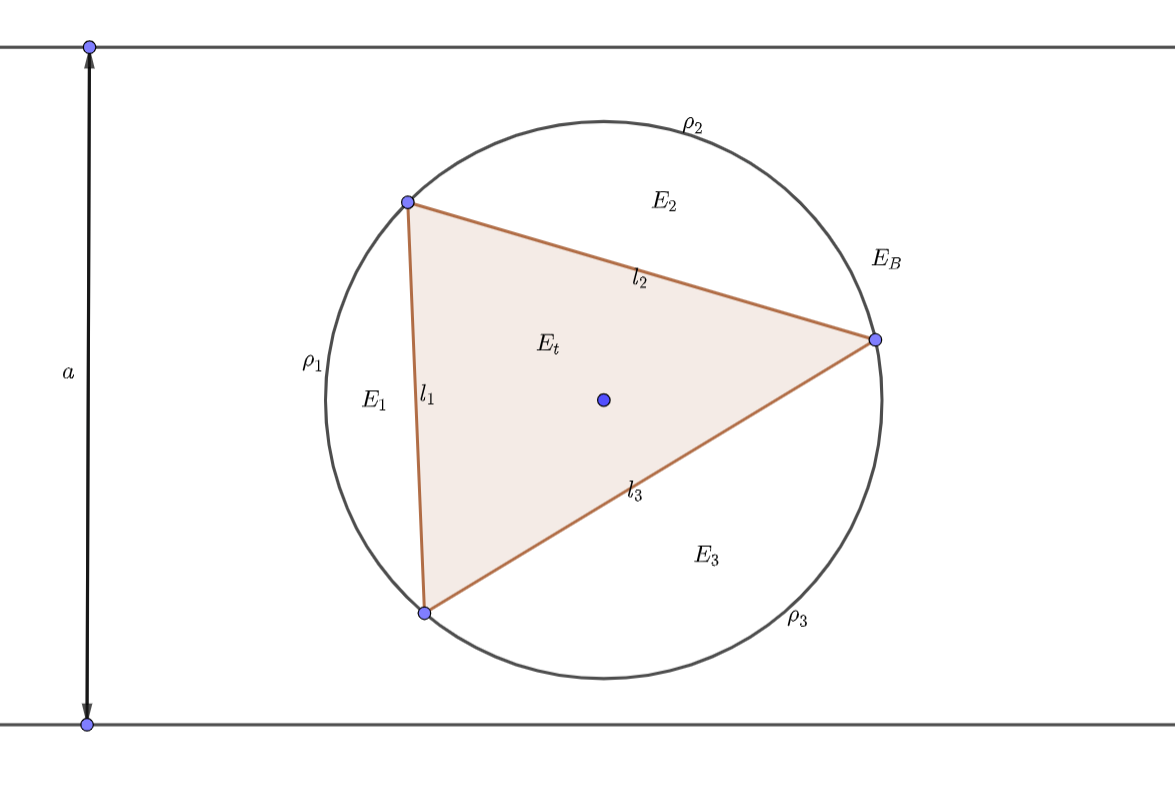
\includegraphics[width=0.8\textwidth]{figure.png}
}
\fi
\iffalse
% 表格模板
\renewcommand\arraystretch{0.8} % 设置表格高度为原来的0.8倍
\begin{table}[!htbp] % table标准
    \centering % 表格居中
    \begin{tabular}{p{1cm}<{\centering}p{1cm}<{\centering}p{3cm}<{\centering}p{5cm}<{\centering}} % 设置表格宽度
    %\begin{tabular}{cccc}
        \toprule
        $x_i$ & $f[x_1]$ & $f[x_i,x_{i+1}]$ & $f[x_i,x_{i+1},x_{i+2}]$ \\
        \midrule
        $x_0$ & $f(x_0)$ &                  &                          \\
        $x_0$ & $f(x_0)$ & $f'(x_0)$        &                          \\
        $x_0$ & $f(x_1)$ & $\frac{f(x_1)-f(x_0)}{x_1-x_0}$ & $\frac{f(x_1)-f(x_0)}{(x_1-x_0)^2}-\frac{f'(x_0)}{x_1-x_0}$\\
        \bottomrule
    \end{tabular}
\end{table}

% 代码块
\begin{lstlisting}
    
\end{lstlisting}
\fi

\end{document}